\chapter{Resultados obtenidos y futuras mejoras}
\label{resultados}

En esta sección se van a comentar los resultados extraídos del proyecto Beerbot. Se debe comenzar comentando que, en última instancia, el trabajo resultó un éxito completo, ya que se alcanzaron los objetivos que se habían planteado. El robot fue capaz de desplazarse por el entorno evitando los obstáculos sin problemas y alcanzando el objetivo asignado. Para poner a prueba el funcionamiento del sistema, se desarrollaron tres escenarios distintos, variando la distribución de los obstáculos. Estos se pueden observar en la figura \ref{escenarios}.\\

\begin{figure}[h]
		\centering
        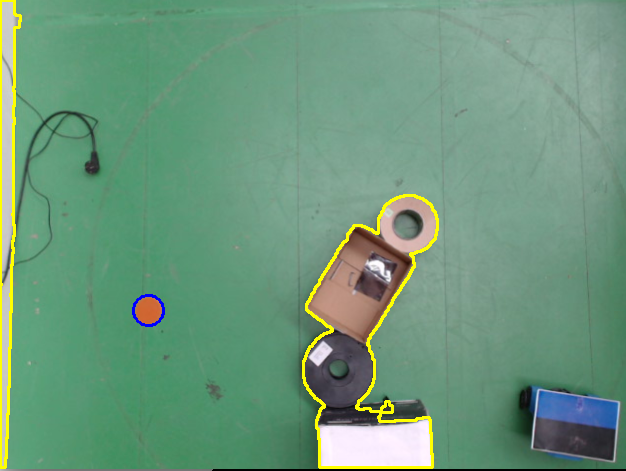
\includegraphics[width=0.35\textwidth]{images/configuration1_segmented.png}
        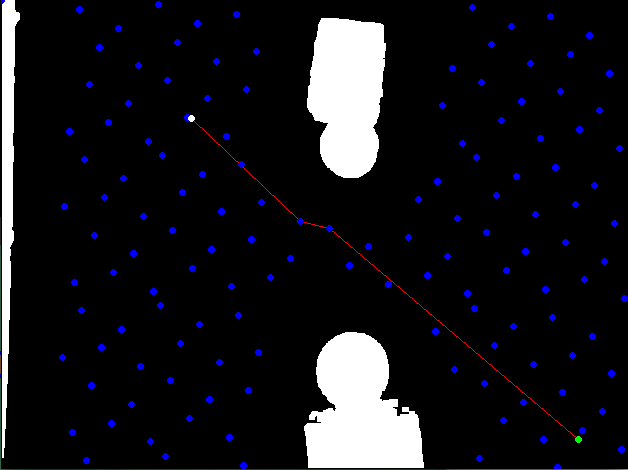
\includegraphics[width=0.35\textwidth]{images/configuration2_trajectory.png}
        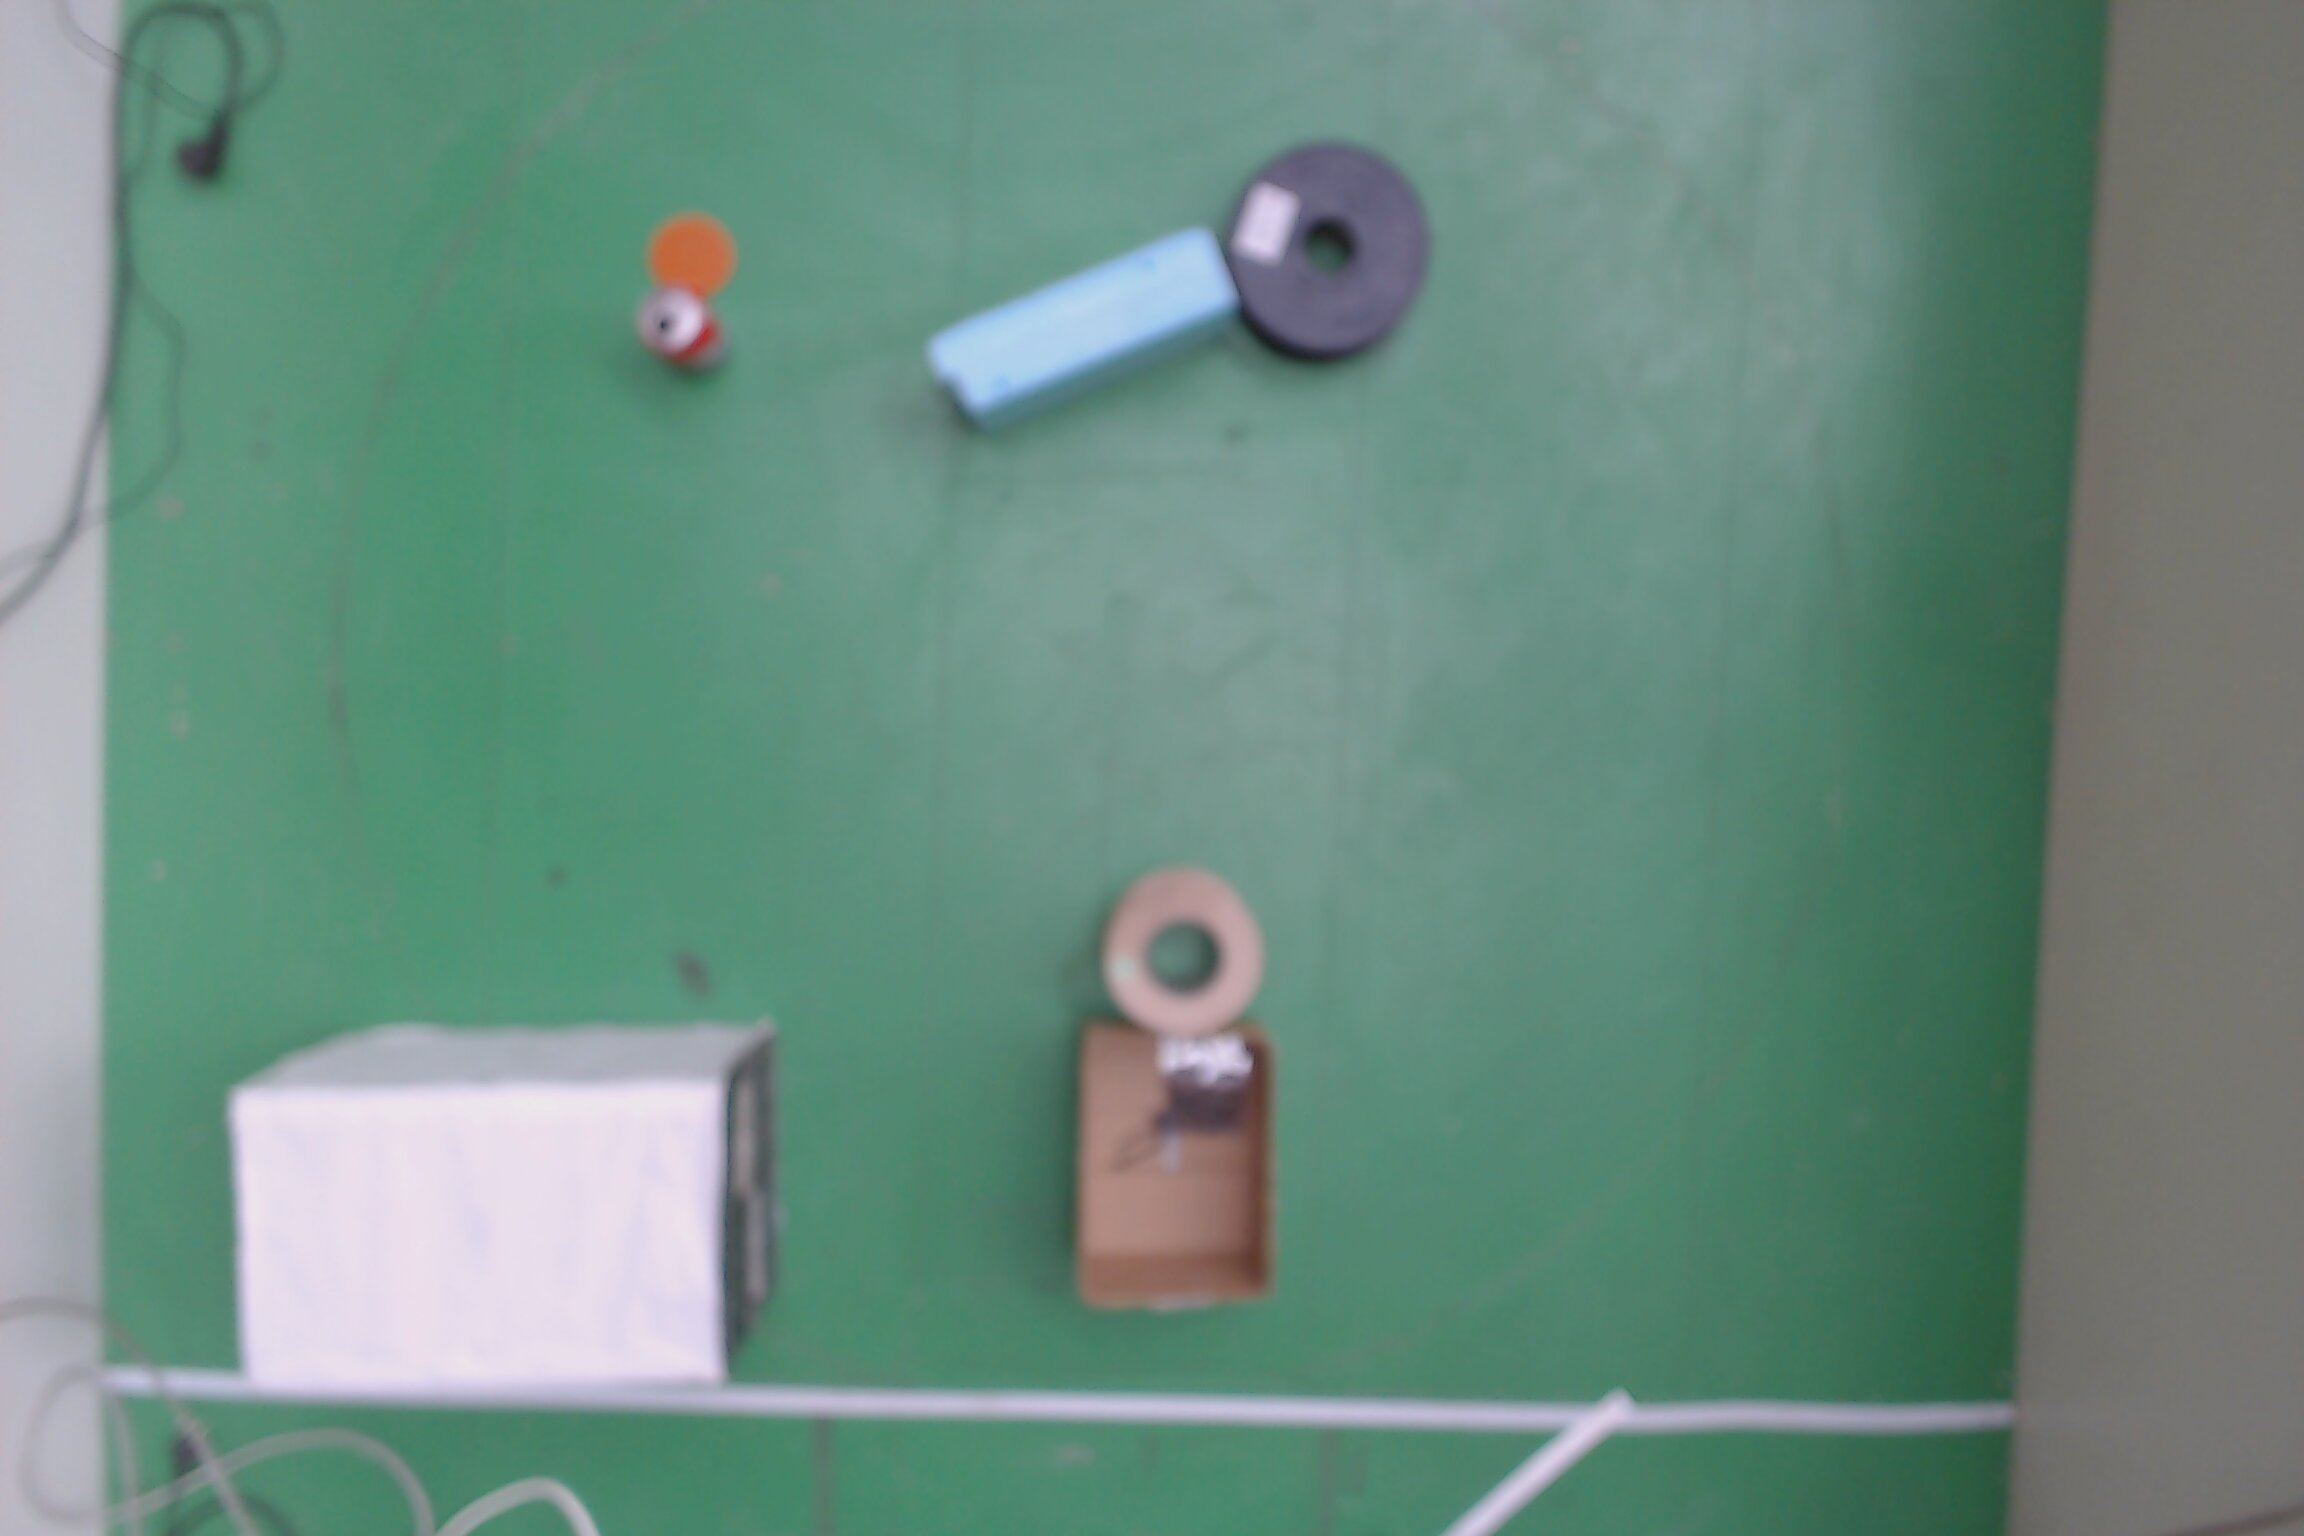
\includegraphics[width=0.35\textwidth]{images/configuration_3.jpg}
        \caption{Escenarios empleados}
        \label{escenarios}
\end{figure}

En los tres entornos el robot fue capaz de alcanzar el punto final sin problemas. Además, se probó a variar la velocidad de avance y se comprobó que, aunque seguía funcionando, podía dar algunos problemas, ya que el sistema necesita pasar por los puntos definidos. En caso de saltarse alguno, el robot se dará la vuelta, irá hasta el nodo que se ha saltado y luego continuará con el camino. En todo caso, este no es un problema fatal, ya que se sigue llegando al lugar deseado, solo supone una cierta pérdida de tiempo. El único caso en el que el robot no fue capaz de alcanzar el objetivo se dió cuando la trayectoria se acercaba demasiado al límite de la imagen que se capta con la cámara. Si el robot en este caso se desvía de la trayectoria y se sale de la zona controlada, pierde la localización, y se queda dando vueltas sobre si mismo. Esto se puede arreglar moviendo manualmente el robot de nuevo a la zona de trabajo.\\

A continuación se comentará como ha funcionado cada una de las partes del sistema en si. Respecto a la parte de procesamiento, inicialmente se planteó de forma distinta a como se ha implementado en la versión final. Se realizaba de igual manera una segmentación del color verde, que corresponde al suelo, en el espacio HSV. A esto se le añadía una segmentación de los colores azul y negro, para eliminar el robot, y del color rojo, para eliminar la lata. La imagen binaria resultante se enviaba al algoritmo de planificación, que se encargaba de extraer los obstáculos y demás. Para la posición y orientación de la lata se segmentaban los colores azul y negro, para encontrar el marcador del robot, y se calculaban los centros de ambas regiones y del marcador en si. Con este último se obtenía la posición del robot, con la orientación del marcador se extraía la dirección de movimiento y con los centros de ambas secciones se extraía el sentido en el que miraba el robot. Cuando esto se llevó a la práctica, se observó que su funcionamiento no era demasiado bueno, ya que los cambios de iluminación provocaban que las segmentaciones no diesen los resultados esperados. Aunque se consiguió filtrar de forma correcta los colores verde, azul y rojo, el color negro fué un problema constante, por lo que se decidió optar por otro enfoque, pasando a la solución explicada en el apartado de software de esta memoria. Con esto se consiguió hacer funcionar de forma adecuada el procesamiento de la imagen.\\

En cuanto al algoritmo de planificación, basta decir que cumplió con su cometido de forma correcta desde el primer momento, al ser un método desarrollado y probado previamente. En este caso no se han hecho estudios en profundidad acerca de como los distintos parámetros del algoritmo afectan a su funcionamiento, pero en caso de estar interesado, dichos estudios se pueden consultar en la memoria contenida en la librería  \textit{PLATANO} \footnote{https://github.com/JavierIH/platano}.\\

Por último, con respecto al sistema de control, fue necesaria una etapa de ajuste durante el proceso de pruebas para conseguir que todo funcionase como es debido. Los principales problemas que se encontraron fueron debidos a los problemas para extraer la orientación del robot debido a la iluminación irregular, que llevaba a una mala segmentación. Al no extraer de forma correcta la orientación, el controlador trataba de reorientar al robot de forma contínua y no era capaz de avanzar. Sin embargo, ajustando la parte de procesamiento de la imagen se consiguió solucionar esto y se consiguió hacer navegar al robot sin más problemas que los ya comentados acerca de la pérdida de localización si este se salía de la zona que capta la imagen y la necesidad de pasar por todos los puntos.\\

Como posibles mejoras al sistema, se ha pensado en dotar al robot de sensores para ser capaz de detectar y evitar obstáculos de forma reactiva, lo que podía ser útil en caso de que un mal ajuste pueda llevar a generar una trayectoria que pase demasiado cerca de un obstáculo. Además de esto, se podría variar el sistema de seguimento de la trayectoria para permitir un movimiento de avance continuó, mientras se va regulando la orientación del robot. Estó permitiría reducir el tiempo que se tarda en alcanzar el objetivo. Por último, si se consigue optimizar los tiempos de procesamiento del entorno y de planificación de trayectoria, se podría utilizar este sistema en entornos donde existiesen obstáculos no estáticos, comprobando cada cierto tiempo si la posición del obstáculo interfiere con la ruta planificada y buscando otro camino en caso de que esto suceda.\\  

La incorporación de un filtro del Kalman u otro sistema estimador de la posición y la orientación también sería una buena incorporación al sistema, ya que se filtrarían los cambios bruscos de posición y orientación producidos por ruido y cambios de iluminación en el sistema de percepción.\\